\PassOptionsToPackage{quiet}{fontspec}
\documentclass[12pt,a4paper,UTF8]{article}
\usepackage{thesis}
\usepackage{indentfirst}
\setlength{\parindent}{2em}
\addtolength{\parskip}{3pt}
\onehalfspacing
\graphicspath{{./figures/}}
\pagestyle{empty}
\usepackage{enumitem}
\usepackage{multirow}
\usepackage{makecell}
\usepackage{url}
\usepackage{float}
\renewcommand{\arraystretch}{1.18}
\setlength{\tabcolsep}{8pt}
\captionsetup[table]{skip=6pt}
\setlength{\textfloatsep}{10pt plus 2pt minus 2pt}
\setlength{\floatsep}{8pt plus 2pt minus 2pt}
\setlength{\intextsep}{8pt plus 2pt minus 2pt}
\newcommand{\FloatBarrier}{\par\smallskip}

\classname{Fundamentals of Optoelectronics}

\begin{document}
\maketitlepage{Solar Cell Design}{Jinghao Shi}{3230100613}{2026.5.26}{Wei Sha}

\newpage

\pagestyle{fancy}
\fancyhf{}
\lhead{Fundamentals of Optoelectronics}
\chead{Solar Cell Design}
\rhead{Jinghao Shi\ 3230100613}
\renewcommand{\headrulewidth}{0.4pt}
\cfoot{\thepage}

\maketoc

\section{Objective}
This project uses the SolarDesign platform to perform coupled optical and electrical simulations of a planar perovskite solar cell. The main objectives are to construct a representative five-layer planar device, analyze the effect of reducing the MAPbI3 active-layer thickness, and compare the FF--$V_\mathrm{oc}$ behavior under different SRH recombination mechanisms. Perovskite solar cells are selected because organometal halide perovskites show strong visible-light absorption and have been widely studied as photovoltaic absorbers \cite{kojima2009,stranks2013,green2016}.

\section{Assignment Requirements}

\begin{enumerate}[label=\arabic*.]
    \item Please calculate the current-density--voltage (\(J\)--\(V\)) curve of a perovskite solar cell with a representative device structure, including five layers: Anode, Cathode, ETL, HTL, and Active layer. All input parameters, including optical and electrical parameters, should be determined. Please study a planar structure without texture. The device structure, band diagram, and \(J\)--\(V\) curve with the characteristic parameters \(J_{\mathrm{sc}}\), \(V_{\mathrm{oc}}\), FF, and PCE should be shown. \hfill [50\%]

    \item Please reduce the thickness of the active layer and investigate the changes in \(J_{\mathrm{sc}}\) short-circuit current, \(V_{\mathrm{oc}}\) open-circuit voltage, FF fill factor, and PCE power conversion efficiency. Please provide physical explanations. Note that only bulk SRH recombination is assumed to exist. \hfill [30\%]

    \item Please calculate the fill factor FF as a function of \(V_{\mathrm{oc}}\). The \(V_{\mathrm{oc}}\) is reduced as the nonradiative SRH recombination increases. Please consider two cases:
    \begin{enumerate}[label=(\arabic*)]
        \item The solar cell has only surface SRH recombination.
        \item The solar cell has only bulk SRH recombination.
    \end{enumerate}
    Please compare the two FF--\(V_{\mathrm{oc}}\) curves corresponding to the two different SRH recombination mechanisms, and explain the difference. \hfill [20\%, difficult]
\end{enumerate}

\section{Key Performance Definitions}
The simulated results are interpreted using the standard photovoltaic definitions below \cite{nelson2003}:
\begin{equation}
    \mathrm{FF}=\frac{J_\mathrm{m}V_\mathrm{m}}{J_\mathrm{sc}V_\mathrm{oc}},
    \qquad
    \mathrm{PCE}=\frac{J_\mathrm{sc}V_\mathrm{oc}\mathrm{FF}}{P_\mathrm{in}},
    \label{eq:ff-pce}
\end{equation}
where $J_\mathrm{m}$ and $V_\mathrm{m}$ are the current density and voltage at the maximum-power point, and $P_\mathrm{in}$ is the incident optical power density.

For trend analysis, the following approximate relations are useful:
\begin{equation}
    J_\mathrm{sc}\propto q\int \Phi(\lambda)A(\lambda)\,d\lambda,
    \label{eq:jsc-abs}
\end{equation}
\begin{equation}
    V_\mathrm{oc}\approx \frac{nk_\mathrm{B}T}{q}
    \ln\left(\frac{J_\mathrm{sc}}{J_0}+1\right).
    \label{eq:voc-j0}
\end{equation}
Here $A(\lambda)$ is the wavelength-dependent absorptance, $\Phi(\lambda)$ is the incident photon flux, and $J_0$ is the dark saturation current density. Therefore, stronger optical absorption tends to increase $J_\mathrm{sc}$, while stronger nonradiative recombination increases $J_0$ and lowers $V_\mathrm{oc}$.

\section{Simulation Results and Discussion}
\subsection{Question 1: Coupled Optical and Electrical Simulation of the Baseline Planar Device}
\subsubsection{Device Structure and Simulation Parameters}
The first optical structure in the SolarDesign public device library, denoted as ``perovskite\_standard'', is selected as the representative planar device. The complete stack is ITO/NiOx/MAPbI3/C60/Ag, corresponding to the anode, hole transport layer, active layer, electron transport layer, and cathode. No texture is introduced, and illumination is assumed to enter from the ITO side.

\begin{table}[H]
    \centering
    \caption{Device structure and layer thicknesses}
    \begin{tabular}{@{}clcc@{}}
        \toprule
        Layer No. & Functional layer & Material & Thickness / nm \\
        \midrule
        1 & Anode & ITO & 50 \\
        2 & Hole transport layer & NiOx & 20 \\
        3 & Active layer & MAPbI3 & 500 \\
        4 & Electron transport layer & C60 & 50 \\
        5 & Cathode & Ag & 120 \\
        \bottomrule
    \end{tabular}
\end{table}

\begin{table}[H]
    \centering
    \caption{Main simulation settings}
    \begin{tabular}{@{}ll@{}}
        \toprule
        Item & Setting \\
        \midrule
        Optical wavelength range & 300--900 nm \\
        Optical wavelength step & 10 nm \\
        Structure type & Planar structure without texture \\
        Operating temperature & 300 K \\
        Recombination mechanism & Bulk SRH recombination only \\
        Electrical simulation mode & Continuous voltage scan \\
        Voltage scan range & 0--1 V \\
        Generation input & From optical simulation result \\
        Illumination intensity & 1 Sun \\
        \bottomrule
    \end{tabular}
\end{table}

The key electrical parameters directly related to the band diagram and carrier transport are summarized in Table \ref{tab:key-elec-params}. ITO and Ag define the contact boundary conditions through their work functions; NiOx and C60 provide selective hole and electron extraction paths; MAPbI3 determines most of the optical absorption and bulk carrier generation. The recombination model follows the Shockley--Read--Hall framework \cite{sze2007}.

\begin{table}[H]
    \centering
    \caption{Key electrical parameters of the device layers}
    \label{tab:key-elec-params}
    \small
    \begin{tabular}{@{}lccccc l@{}}
        \toprule
        Layer & $\varepsilon_r$ & $\mu_n$ & $\mu_p$ & $\chi$ (eV) & $E_g$ (eV) & Note \\
        \midrule
        ITO & -- & -- & -- & -- & -- & WF = 5.4 eV \\
        NiOx & 4 & $1\times10^{-2}$ & 20 & 3.6 & 1.8 & $\tau_n=\tau_p=10^6$ s \\
        MAPbI3 & 31 & 20 & 20 & 3.9 & 1.5 & $\tau_n=\tau_p=10^{-5}$ s \\
        C60 & 4 & 20 & $1\times10^{-2}$ & 3.9 & 1.8 & $\tau_n=\tau_p=10^6$ s \\
        Ag & -- & -- & -- & -- & -- & WF = 3.9 eV \\
        \bottomrule
    \end{tabular}
\end{table}

\begin{figure}[H]
    \centering
    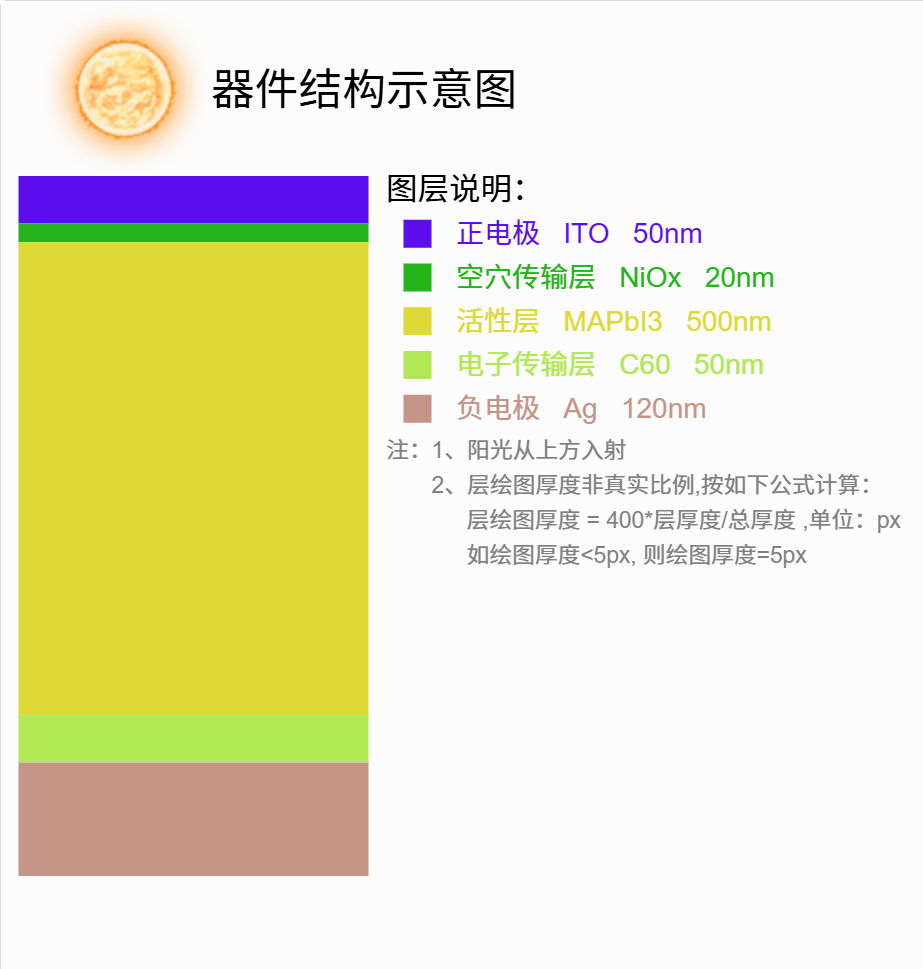
\includegraphics[width=0.82\textwidth]{器件结构示意图.png}
    \caption{Schematic structure of the baseline planar device}
\end{figure}

\FloatBarrier

\subsubsection{Optical Simulation Results}
Based on the complex refractive indices and layer thicknesses above, the optical simulation is performed first. Figure \ref{fig:absorption} shows the absorption spectrum of the device.

The device has high absorption in the visible range. The absorption increases significantly from about 500 nm, remains above 0.9 over most of the 530--750 nm range, and reaches a peak close to 0.98 near 690--710 nm. When the wavelength approaches 780--790 nm, the absorption drops rapidly, corresponding to the band-edge absorption of MAPbI3 \cite{dewolf2014}.

\begin{figure}[H]
    \centering
    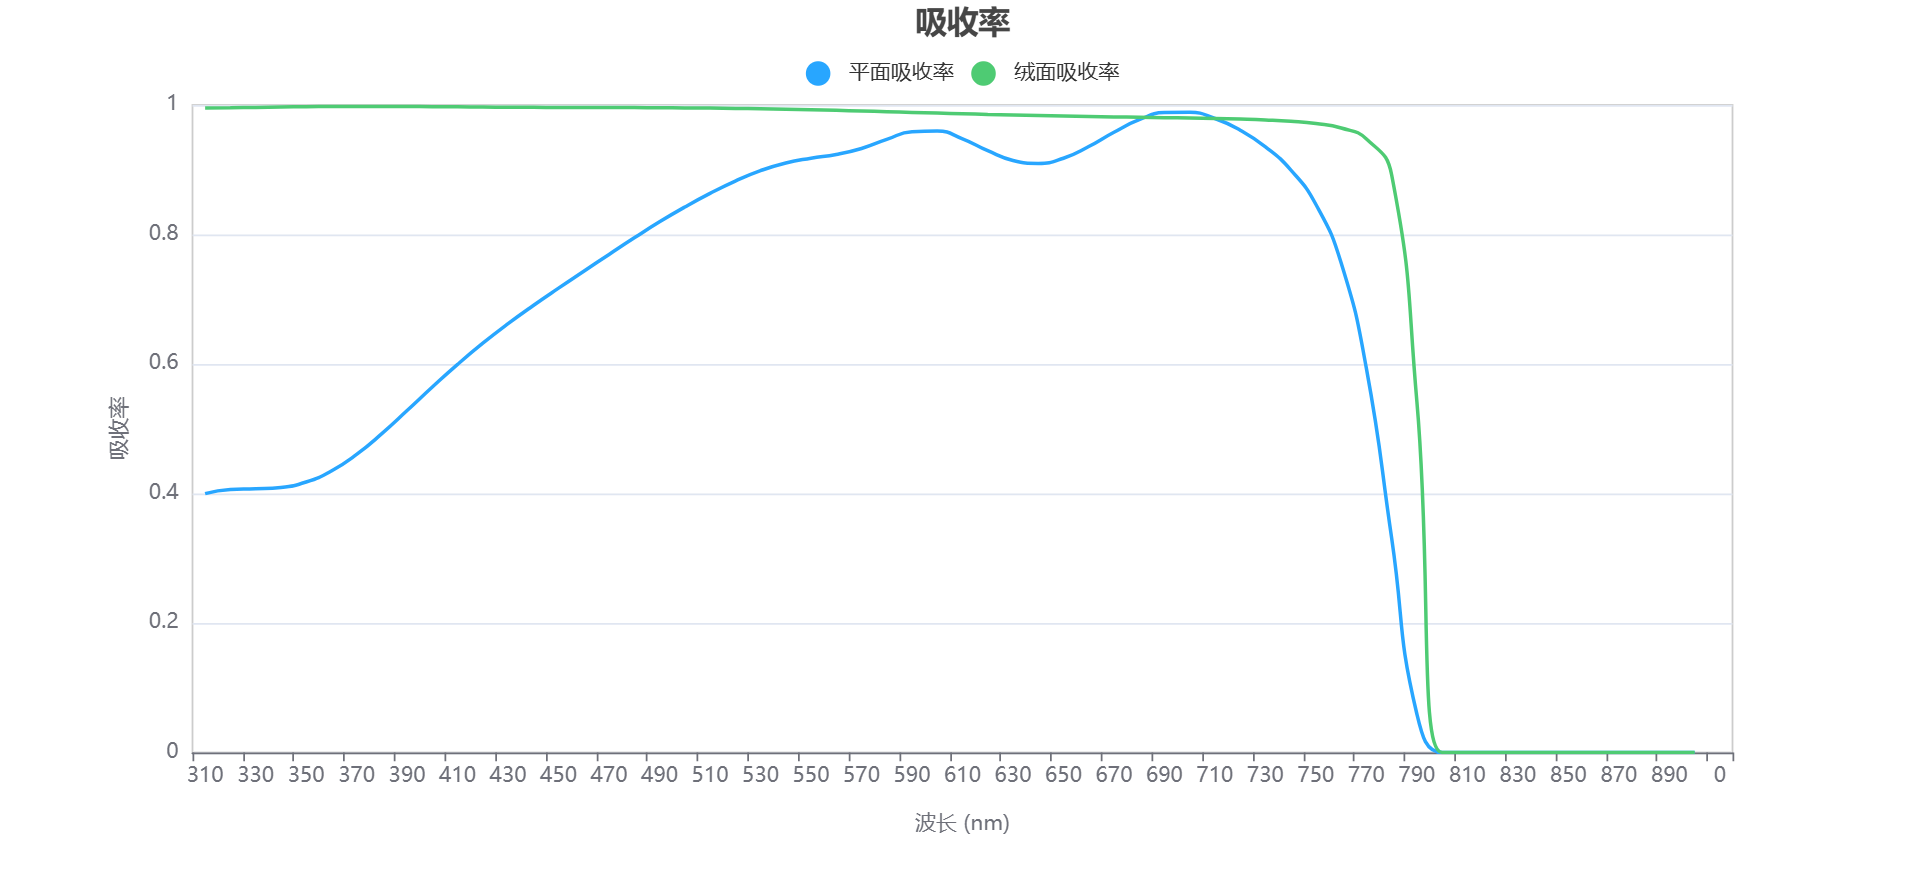
\includegraphics[width=0.86\textwidth]{吸收率.png}
    \caption{Absorption spectrum of the baseline device}
    \label{fig:absorption}
\end{figure}

Figure \ref{fig:ref-tra} further shows the wavelength-dependent reflectance and transmittance. For a planar thin-film stack,
\begin{equation}
    A(\lambda)+R(\lambda)+T(\lambda)=1.
    \label{eq:art}
\end{equation}
Because the bottom Ag electrode blocks transmitted light strongly, $T(\lambda)$ is close to zero throughout the simulated wavelength range. Thus, photons not absorbed by the device are mainly lost through reflection. The reflectance remains low in the main absorption range of 530--750 nm and reaches a minimum near 700 nm. Beyond the MAPbI3 absorption edge, absorption decreases and reflectance rises sharply. This thin-film optical behavior is consistent with the transfer-matrix description of multilayer solar-cell optics \cite{pettersson1999}.

\begin{figure}[H]
    \centering
    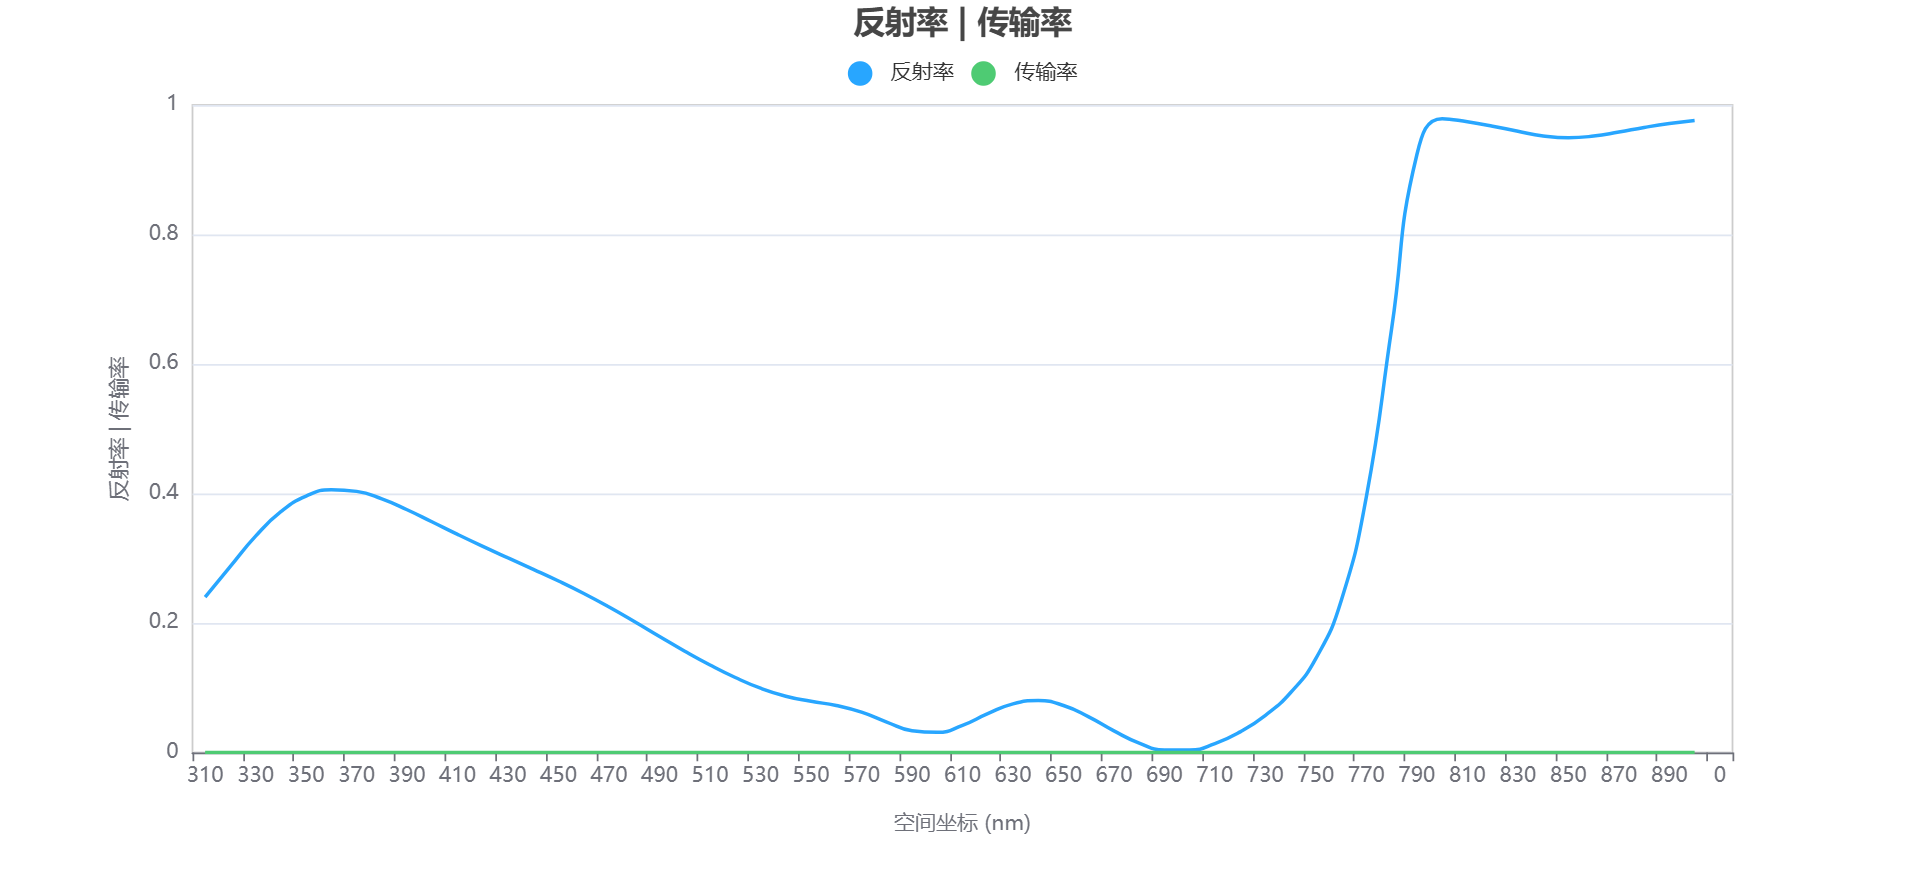
\includegraphics[width=0.86\textwidth]{反射率 _ 传输率.png}
    \caption{Reflectance and transmittance spectra of the baseline device}
    \label{fig:ref-tra}
\end{figure}

The generation-rate distribution gives the spatial origin of the photocurrent. Photogenerated carriers are mainly produced near the incident side, and the generation rate gradually decreases along the device thickness because fewer photons remain available deeper in the stack. The optical simulation gives the limiting short-circuit current density as
\[
J_{\mathrm{sc,limit}} = 21.6823\ \mathrm{mA/cm^2}.
\]
This value can be used as an optical upper reference for the electrical-simulation result of $J_\mathrm{sc}$.

\begin{figure}[H]
    \centering
    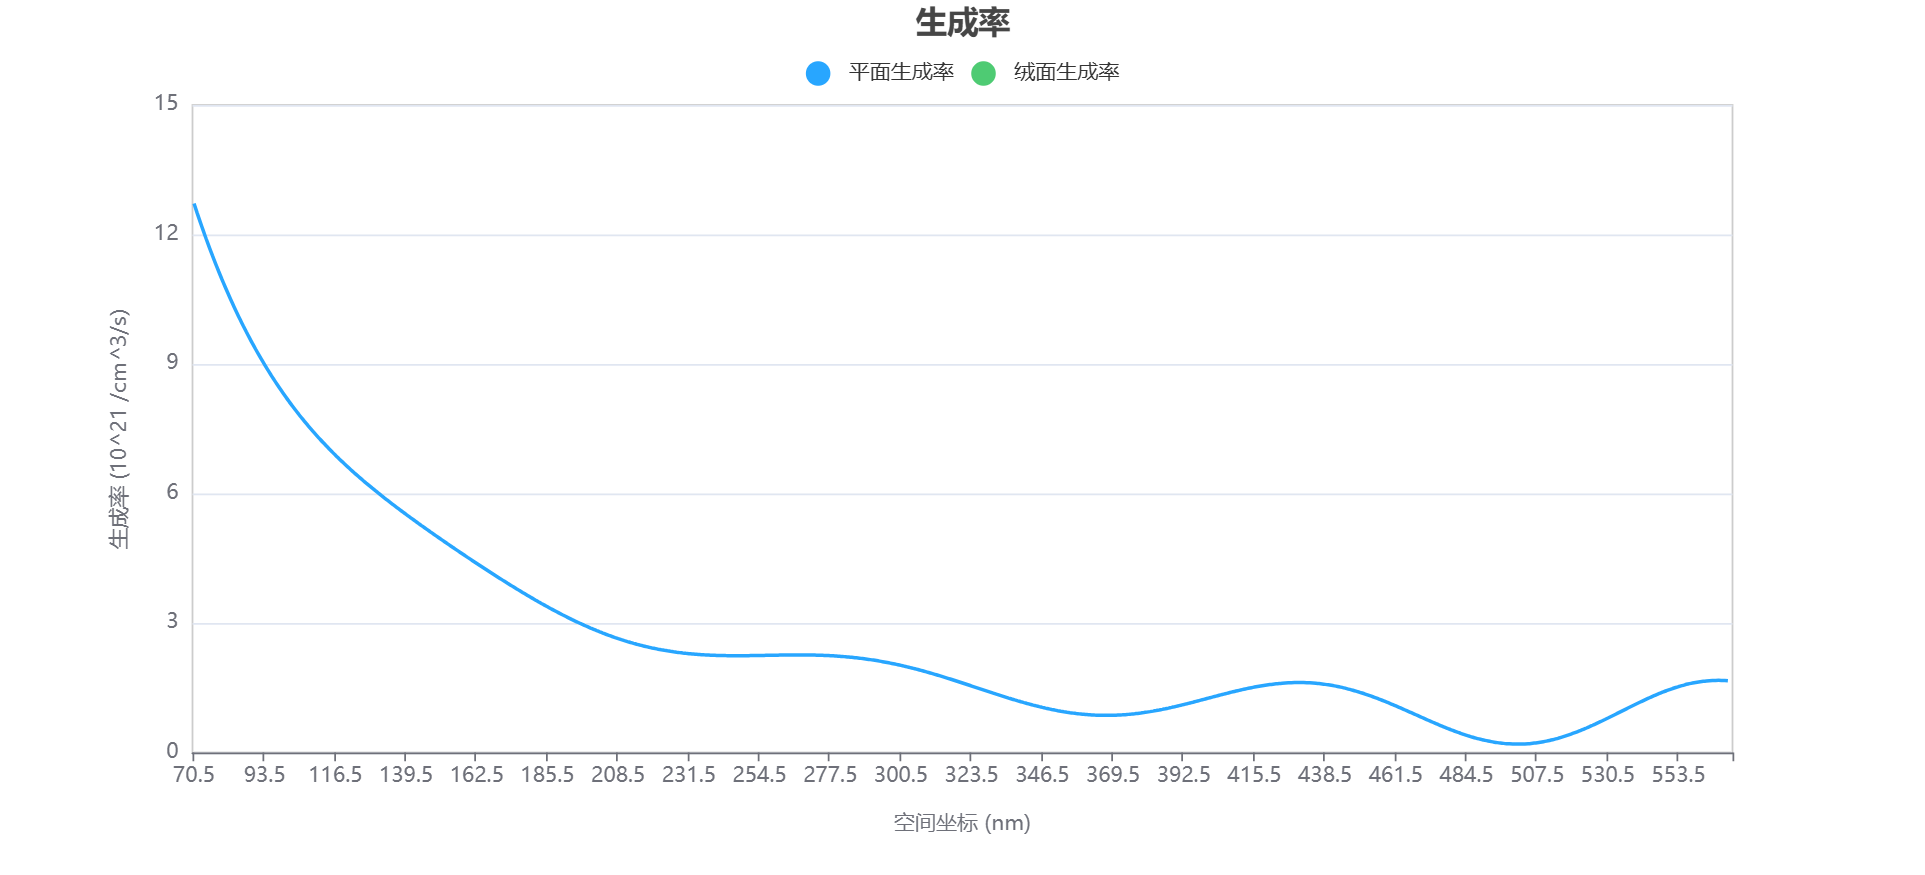
\includegraphics[width=0.86\textwidth]{生成率.png}
    \caption{Internal photogeneration-rate distribution}
    \label{fig:generation}
\end{figure}

\FloatBarrier

\subsubsection{Electrical Simulation Results}
After importing the optical generation profile, the electrical simulation is performed. Figure \ref{fig:band} shows the energy-band diagram of the device.

NiOx acts as the hole transport layer, and its deeper energy level favors hole extraction. C60 acts as the electron transport layer and forms an electron-selective interface with MAPbI3. The work functions of ITO and Ag are 5.4 eV and 3.9 eV, respectively. Overall, the band alignment supports carrier separation and selective collection.

\begin{figure}[H]
    \centering
    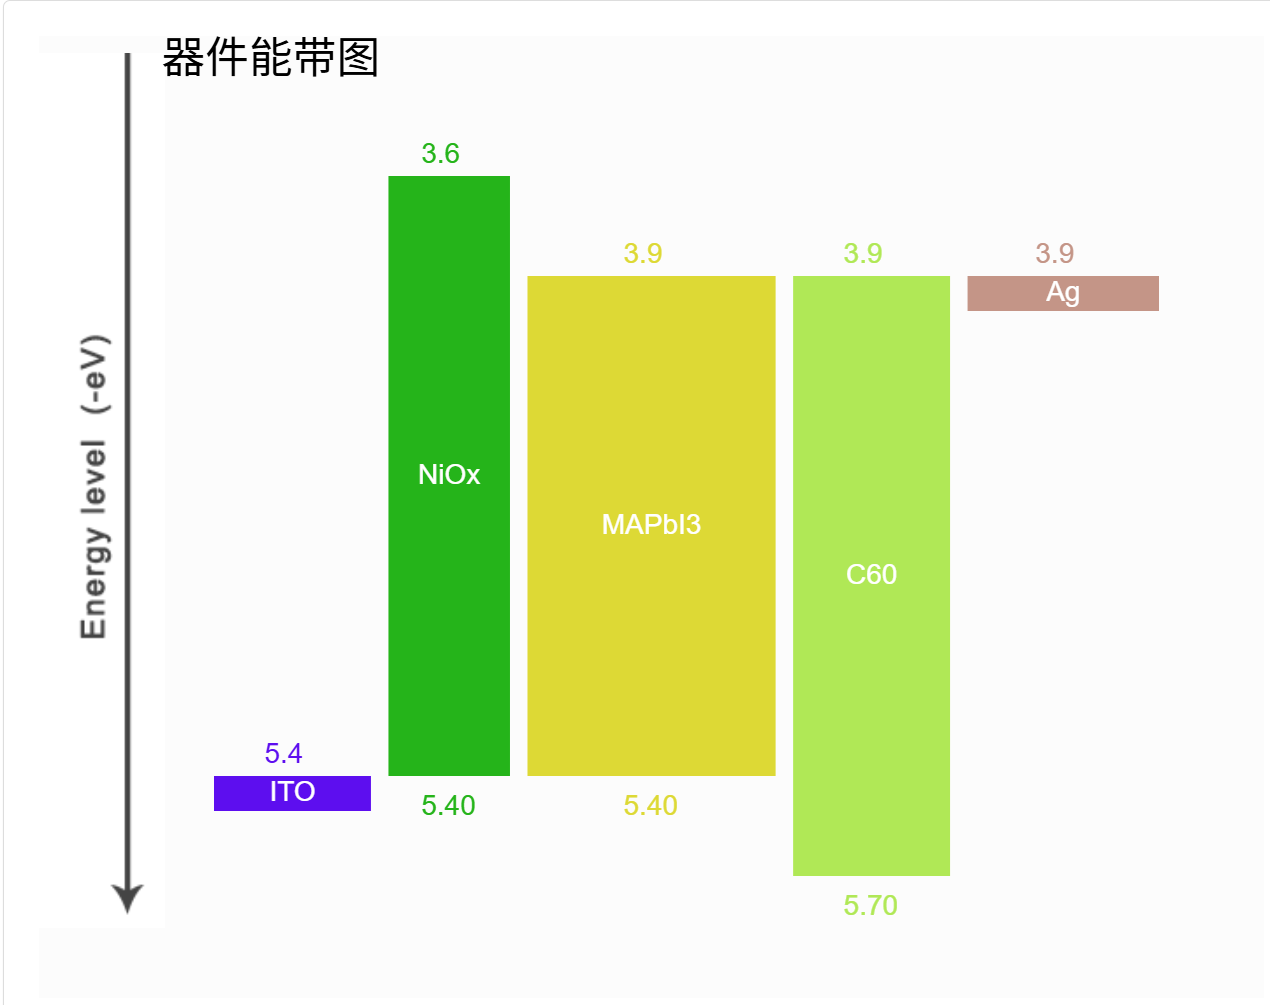
\includegraphics[width=0.78\textwidth]{器件能带图.png}
    \caption{Energy-band diagram of the baseline device}
    \label{fig:band}
\end{figure}

The corresponding $J$--$V$ curve is shown in Figure \ref{fig:jv}. The current density remains high and nearly flat at low voltage, then decreases rapidly near the open-circuit voltage. The characteristic parameters exported by the platform are
\[
J_\mathrm{sc} = 21.6822\ \mathrm{mA/cm^2},\quad
V_\mathrm{oc} = 0.993\ \mathrm{V},
\]
\[
\mathrm{FF} = 80.7154\%,\quad
\mathrm{PCE} = 17.3783\%.
\]

\begin{figure}[H]
    \centering
    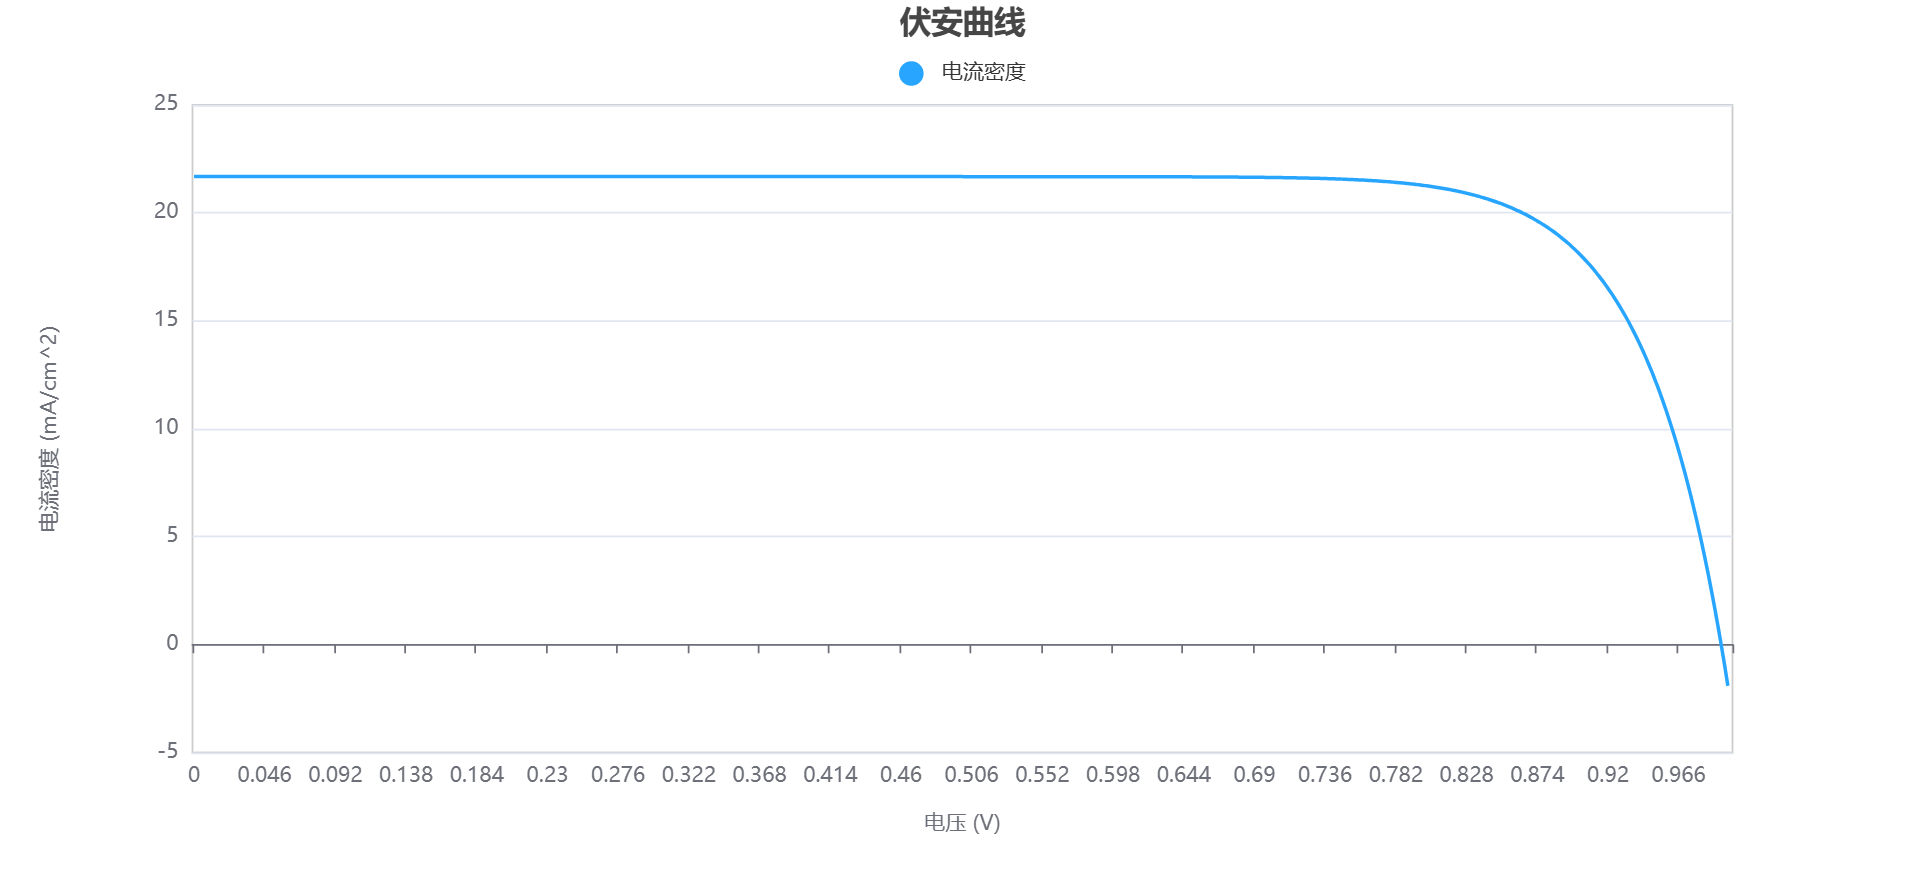
\includegraphics[width=0.86\textwidth]{伏安曲线.png}
    \caption{$J$--$V$ curve of the baseline device}
    \label{fig:jv}
\end{figure}

\begin{table}[H]
    \centering
    \caption{Electrical performance parameters of the baseline device}
    \begin{tabular}{@{}cccc@{}}
        \toprule
        $J_\mathrm{sc}$ / $\mathrm{mA/cm^2}$ & $V_\mathrm{oc}$ / V & FF / \% & PCE / \% \\
        \midrule
        21.6822 & 0.993 & 80.7154 & 17.3783 \\
        \bottomrule
    \end{tabular}
\end{table}

The electrical $J_\mathrm{sc}$ is almost identical to the optical limiting current density, so the current loss from carrier transport and collection is small. This indicates that $J_\mathrm{sc}$ is mainly controlled by optical absorption, as described by Eq. \eqref{eq:jsc-abs}. In contrast, $V_\mathrm{oc}$ and FF are more sensitive to recombination, band alignment, and electrical transport losses. The obtained PCE follows directly from Eq. \eqref{eq:ff-pce}, which is consistent with the standard interpretation of photovoltaic performance parameters \cite{shockley1961,green2016}.

\FloatBarrier

\subsubsection{Summary of Question 1}
For Question 1, the required device structure, optical results, band diagram, $J$--$V$ curve, and characteristic parameters have all been obtained. The baseline device gives $J_\mathrm{sc}=21.6822\ \mathrm{mA/cm^2}$, $V_\mathrm{oc}=0.993$ V, FF = 80.7154\%, and PCE = 17.3783\%. This structure is used as the baseline for the subsequent active-layer thickness study and FF--$V_\mathrm{oc}$ analysis.

\subsection{Question 2: Effect of Active-Layer Thickness on Device Performance}
For Question 2, only the MAPbI3 active-layer thickness is changed. The ITO, NiOx, C60, and Ag layers remain unchanged, and only bulk SRH recombination is included according to the assignment requirement. For each thickness point, optical simulation is performed first, and the corresponding generation-rate profile is then imported into the electrical simulation.

\subsubsection{Thickness-Scan Results}
Using the 500 nm active layer in Question 1 as the baseline, the MAPbI3 thickness is reduced to 400 nm, 300 nm, 200 nm, and 100 nm. The characteristic parameters exported by the platform are shown together in Figure \ref{fig:q2-screenshots}, and the extracted data are summarized in Table \ref{tab:thickness-scan}.

\begin{figure}[H]
    \centering
    \begin{subfigure}{0.49\textwidth}
        \centering
        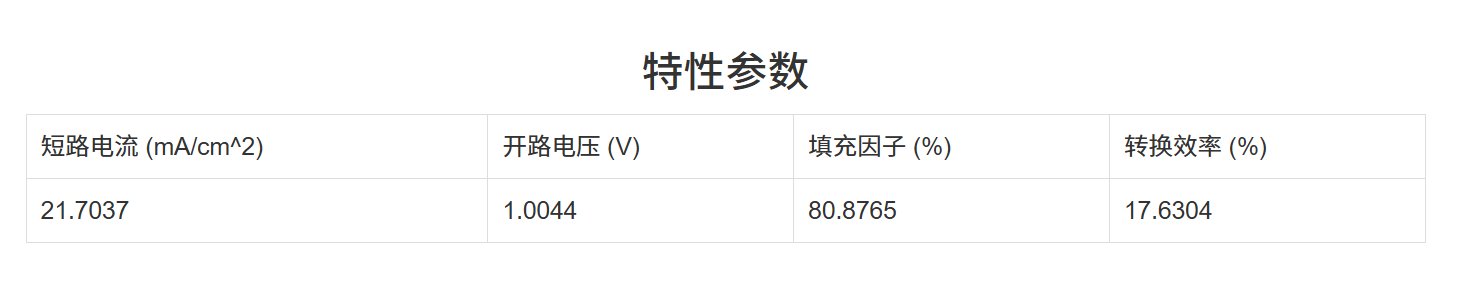
\includegraphics[width=\textwidth]{400nm.png}
        \caption{400 nm}
        \label{fig:q2-400}
    \end{subfigure}
    \hfill
    \begin{subfigure}{0.49\textwidth}
        \centering
        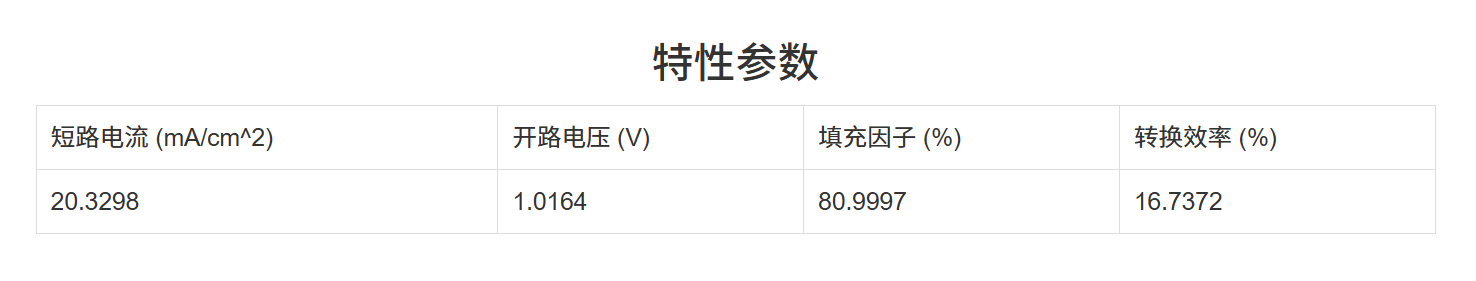
\includegraphics[width=\textwidth]{300nm.png}
        \caption{300 nm}
        \label{fig:q2-300}
    \end{subfigure}

    \vspace{0.2cm}

    \begin{subfigure}{0.49\textwidth}
        \centering
        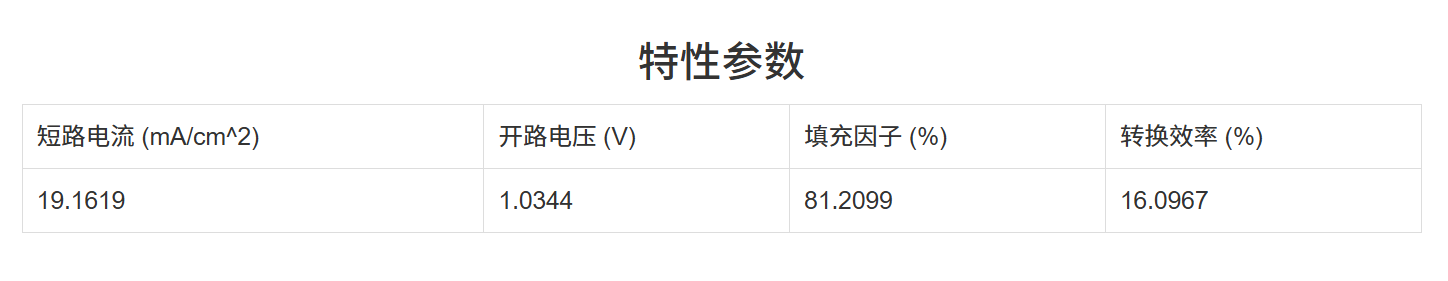
\includegraphics[width=\textwidth]{200nm.png}
        \caption{200 nm}
        \label{fig:q2-200}
    \end{subfigure}
    \hfill
    \begin{subfigure}{0.49\textwidth}
        \centering
        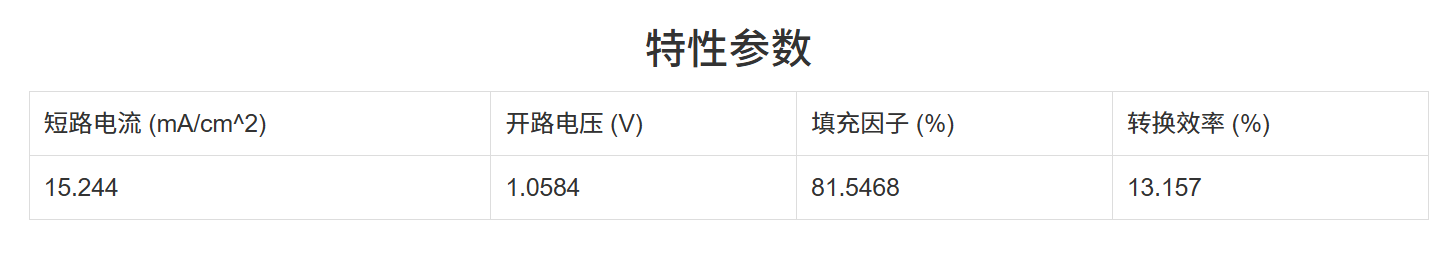
\includegraphics[width=\textwidth]{100nm.png}
        \caption{100 nm}
        \label{fig:q2-100}
    \end{subfigure}
    \caption{Characteristic parameters exported by the platform for different MAPbI3 active-layer thicknesses}
    \label{fig:q2-screenshots}
\end{figure}

\FloatBarrier

\begin{table}[H]
    \centering
    \caption{Device performance parameters at different MAPbI3 active-layer thicknesses}
    \label{tab:thickness-scan}
    \begin{tabular}{@{}ccccc@{}}
        \toprule
        Thickness / nm & $J_\mathrm{sc}$ / $\mathrm{mA/cm^2}$ & $V_\mathrm{oc}$ / V & FF / \% & PCE / \% \\
        \midrule
        500 & 21.6822 & 0.9930 & 80.7154 & 17.3783 \\
        400 & 21.7037 & 1.0044 & 80.8765 & 17.6304 \\
        300 & 20.3298 & 1.0164 & 80.9997 & 16.7372 \\
        200 & 19.1619 & 1.0344 & 81.2099 & 16.0967 \\
        100 & 15.2440 & 1.0584 & 81.5468 & 13.1570 \\
        \bottomrule
    \end{tabular}
\end{table}

The thickness dependences of the four performance parameters are plotted separately in Figure \ref{fig:q2-thickness-curves}. The original units are used in each subfigure so that the absolute variations of $J_\mathrm{sc}$, $V_\mathrm{oc}$, FF, and PCE can be read directly.

\FloatBarrier

\begin{figure}[H]
    \centering
    \begin{subfigure}{0.48\textwidth}
        \centering
        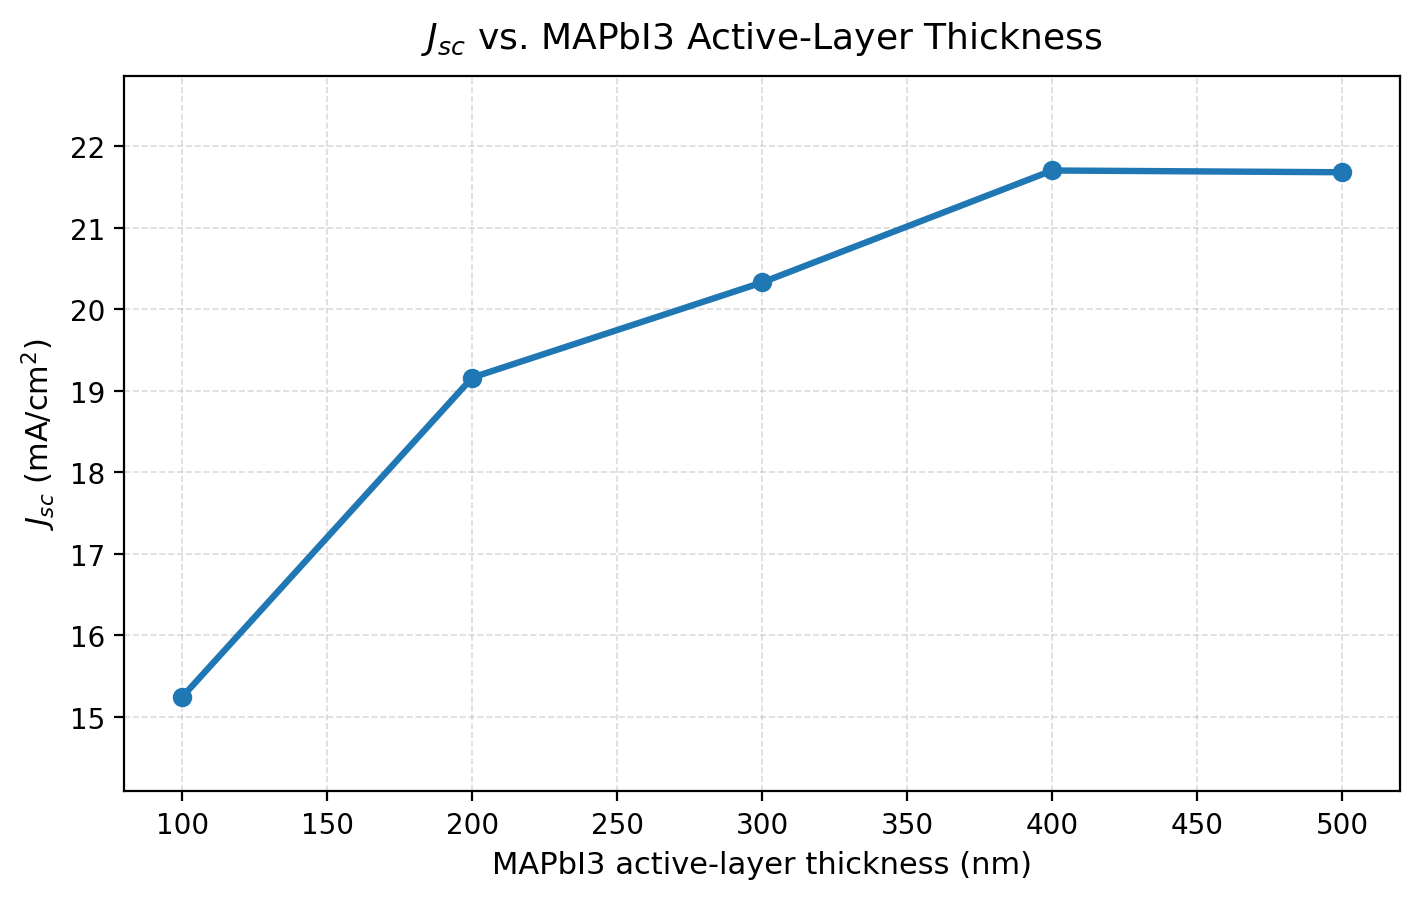
\includegraphics[width=\textwidth]{q2_jsc_vs_thickness.png}
        \caption{$J_\mathrm{sc}$}
    \end{subfigure}
    \hfill
    \begin{subfigure}{0.48\textwidth}
        \centering
        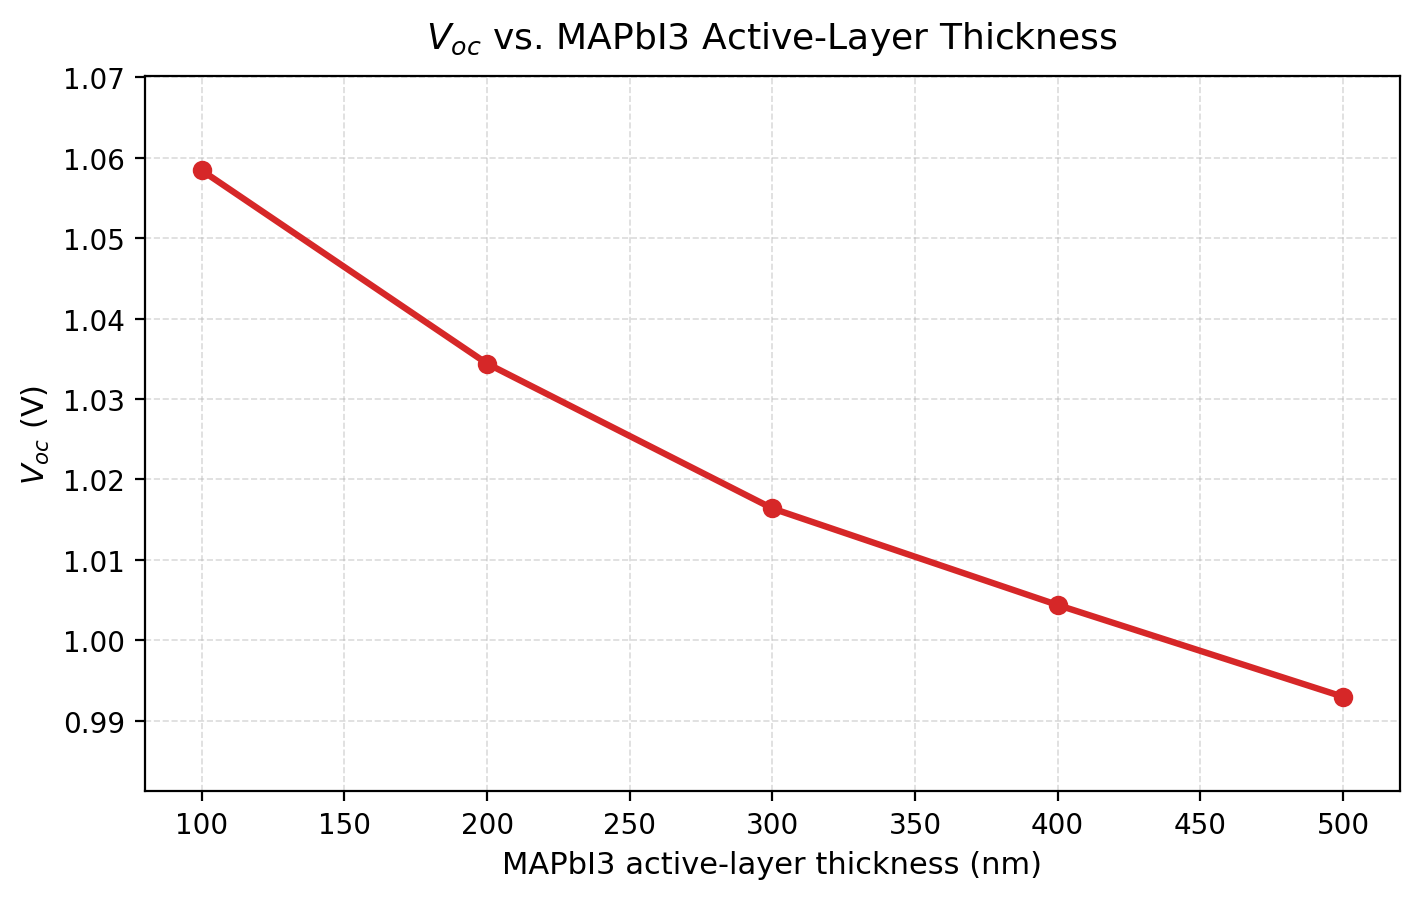
\includegraphics[width=\textwidth]{q2_voc_vs_thickness.png}
        \caption{$V_\mathrm{oc}$}
    \end{subfigure}

    \vspace{0.3cm}

    \begin{subfigure}{0.48\textwidth}
        \centering
        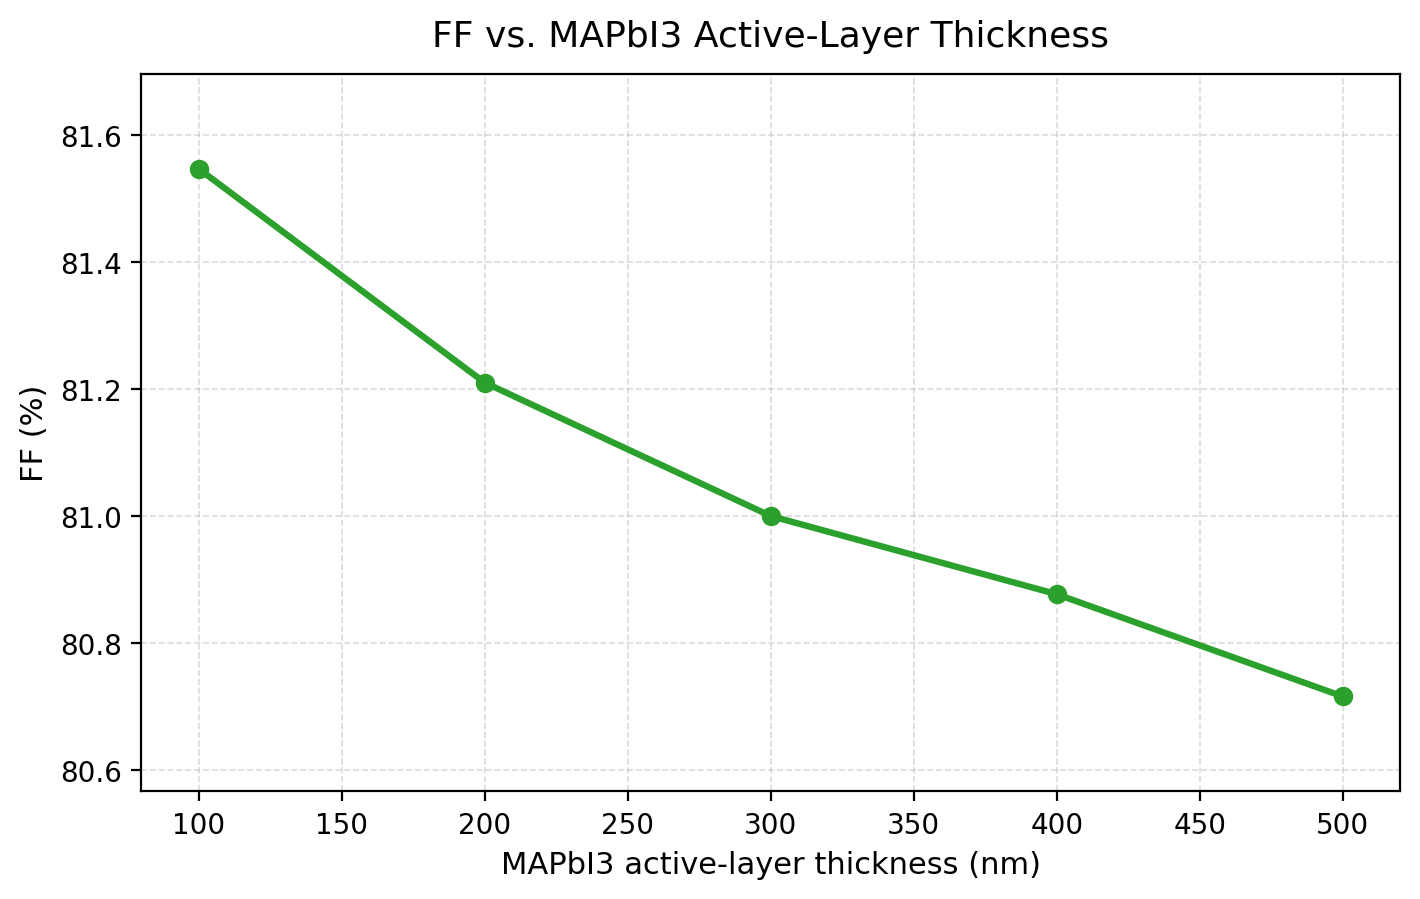
\includegraphics[width=\textwidth]{q2_ff_vs_thickness.png}
        \caption{FF}
    \end{subfigure}
    \hfill
    \begin{subfigure}{0.48\textwidth}
        \centering
        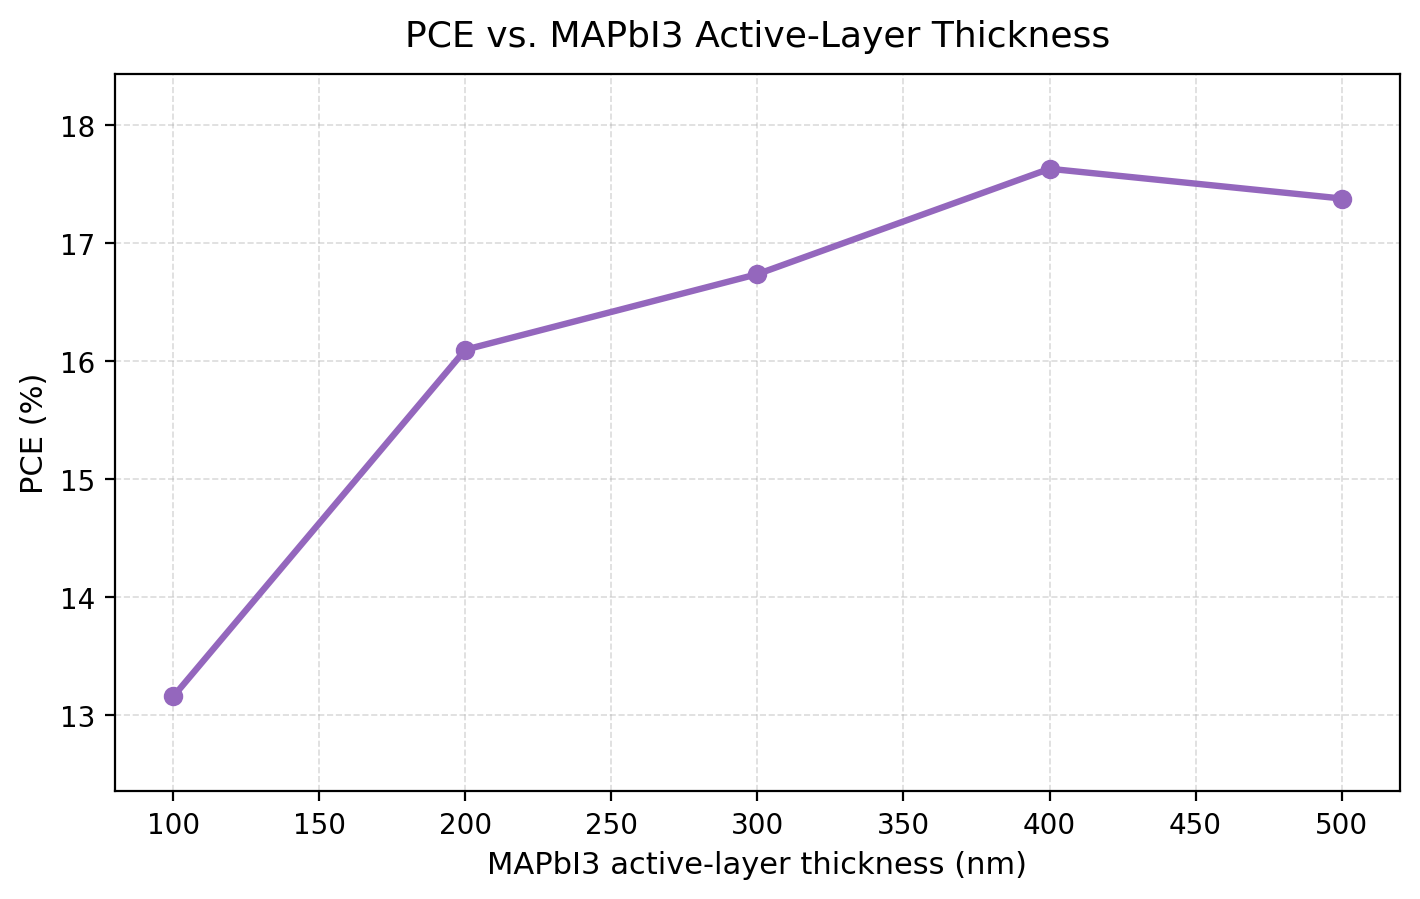
\includegraphics[width=\textwidth]{q2_pce_vs_thickness.png}
        \caption{PCE}
    \end{subfigure}
    \caption{Thickness dependence of $J_\mathrm{sc}$, $V_\mathrm{oc}$, FF, and PCE using the original units}
    \label{fig:q2-thickness-curves}
\end{figure}

\FloatBarrier

\subsubsection{Physical Explanation}
Table \ref{tab:thickness-scan} and Figure \ref{fig:q2-thickness-curves} show a trade-off between optical absorption and recombination loss. The main trend can be explained from three aspects.

\begin{enumerate}[label=\textbf{\arabic*.}]
    \item \textbf{$J_\mathrm{sc}$ decreases for thin absorbers.}
    
    A thinner MAPbI3 layer provides a shorter absorption path, especially for photons near the long-wavelength absorption edge. Therefore, the absorbed photon flux in Eq. \eqref{eq:jsc-abs} decreases. This explains the reduction of $J_\mathrm{sc}$ from 21.6822 $\mathrm{mA/cm^2}$ at 500 nm to 15.2440 $\mathrm{mA/cm^2}$ at 100 nm. The 400 nm result is very close to the 500 nm result; the small difference can be attributed to thin-film interference and numerical variation.

    \item \textbf{$V_\mathrm{oc}$ and FF increase slightly.}
    
    With only bulk SRH recombination included, reducing the absorber thickness reduces the bulk recombination volume and shortens the average carrier transport distance. The dark recombination current $J_0$ is therefore reduced, and Eq. \eqref{eq:voc-j0} gives a larger $V_\mathrm{oc}$. In the simulation, $V_\mathrm{oc}$ increases from 0.9930 V at 500 nm to 1.0584 V at 100 nm. FF also rises slightly from 80.7154\% to 81.5468\%, indicating that carrier extraction becomes slightly easier in the thinner device.

    \item \textbf{PCE has an optimum thickness.}
    
    From Eq. \eqref{eq:ff-pce}, PCE depends on the product $J_\mathrm{sc}V_\mathrm{oc}\mathrm{FF}$. At 400 nm, $V_\mathrm{oc}$ and FF increase while $J_\mathrm{sc}$ remains almost unchanged, so PCE improves slightly to 17.6304\%. Below 300 nm, the loss in $J_\mathrm{sc}$ dominates, and PCE decreases. Among the simulated cases, 400 nm gives the best performance.
\end{enumerate}

\clearpage

\subsection{Question 3: FF--$V_\mathrm{oc}$ Relationship and the Effect of SRH Recombination}
This part compares how FF changes with $V_\mathrm{oc}$ when nonradiative SRH recombination is strengthened. Stronger SRH recombination reduces the nonequilibrium carrier density and decreases the splitting between the electron and hole quasi-Fermi levels, so $V_\mathrm{oc}$ decreases. At the same time, the maximum-power region of the $J$--$V$ curve changes, so FF is also affected \cite{tress2017}.

\subsubsection{Simulation Principle and Parameter Settings}
For bulk SRH recombination, the recombination rate is described by \cite{shockley1952,hall1952,sze2007}
\begin{equation}
    U_\mathrm{SRH}=
    \frac{np-n_i^2}
    {\tau_p(n+n_1)+\tau_n(p+p_1)}.
    \label{eq:srh}
\end{equation}
Thus, a shorter lifetime $\tau$ means stronger nonradiative recombination. In the surface-SRH-dominant approximation used here, the intended recombination loss is concentrated near the interfaces rather than distributed uniformly in the absorber.

The device structure and optical generation profile are kept the same as those of the 500 nm baseline device in Question 1. Only the SRH-related electrical parameters are scanned:

\begin{enumerate}[label=(\arabic*)]
    \item \textbf{Bulk SRH recombination:} surface SRH and Auger recombination are disabled, and only bulk SRH recombination is enabled. The electron and hole lifetimes in the MAPbI3 active layer are set equal and scanned from $10^{-3}$ s to $10^{-9}$ s.
    \item \textbf{Surface-SRH-dominant approximation:} the assignment asks for the ``only surface SRH'' case. However, in the SolarDesign platform, selecting surface SRH requires bulk SRH to be enabled at the same time. Therefore, this case is implemented by enabling both surface SRH and bulk SRH, while setting the bulk lifetimes to very large values so that bulk recombination is negligible. In the following discussion, this setting is referred to as the surface-SRH-dominant case, which approximates the only-surface-SRH condition rather than representing a strictly pure surface-only model. The surface-related lifetime at the active-layer interfaces is scanned from $10^2$ s to $10^{-9}$ s.
\end{enumerate}

The corresponding electrical-parameter settings are shown in Figure \ref{fig:q3-settings}. For both scans, the voltage range is chosen large enough to include the open-circuit voltage.

\begin{figure}[H]
    \centering
    \begin{subfigure}{0.48\textwidth}
        \centering
        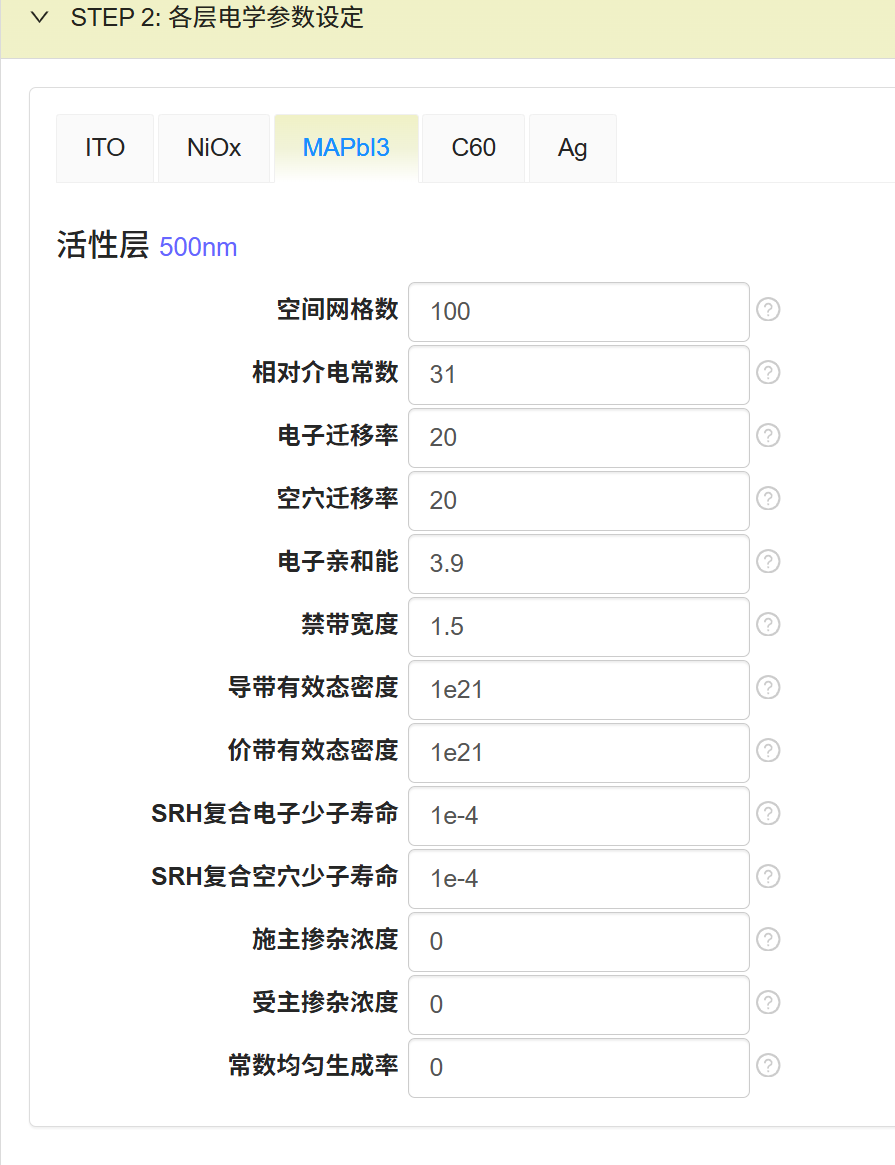
\includegraphics[width=\textwidth]{q3调整电学参数_体复合τ.png}
        \caption{Bulk SRH lifetime scan}
    \end{subfigure}
    \hfill
    \begin{subfigure}{0.48\textwidth}
        \centering
        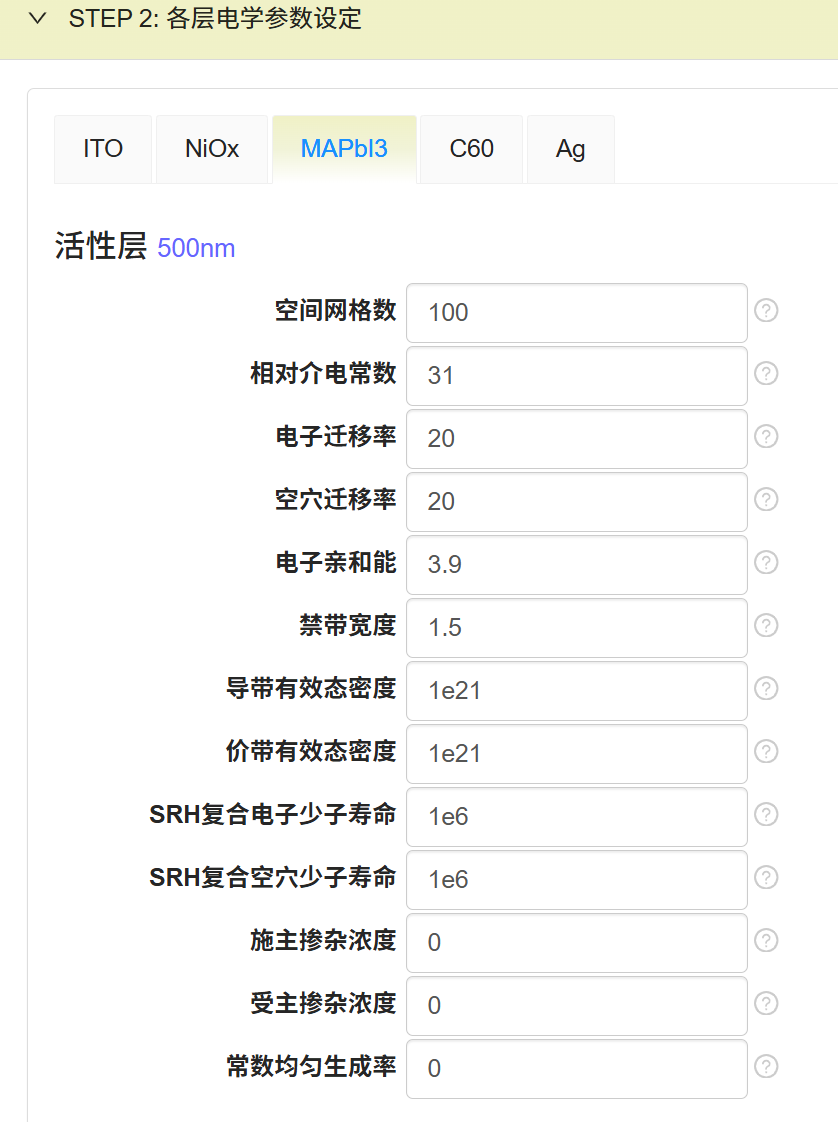
\includegraphics[width=\textwidth]{q3调整电学参数_表面复合的活性层τ.png}
        \caption{Surface-SRH-dominant approximation scan}
    \end{subfigure}
    \caption{Electrical-parameter settings used for the SRH recombination scans}
    \label{fig:q3-settings}
\end{figure}

\FloatBarrier

\subsubsection{Bulk SRH Recombination Results}
Table \ref{tab:q3-bulk} summarizes the extracted $V_\mathrm{oc}$ and FF values for the bulk SRH scan. As $\tau_n=\tau_p$ decreases, the bulk SRH recombination rate increases according to Eq. \eqref{eq:srh}. As a result, $V_\mathrm{oc}$ decreases from 1.2285 V to 0.5681 V, and FF decreases from 83.1317\% to 65.7934\%. The FF loss becomes especially strong when $V_\mathrm{oc}$ falls below about 0.7 V.

\begin{table}[H]
    \centering
    \caption{FF--$V_\mathrm{oc}$ data for the bulk SRH recombination scan}
    \label{tab:q3-bulk}
    \small
    \begin{tabular}{@{}ccc@{}}
        \toprule
        Bulk lifetime $\tau_n=\tau_p$ / s & $V_\mathrm{oc}$ / V & FF / \% \\
        \midrule
        $1\times10^{-3}$ & 1.2285 & 83.1317 \\
        $5\times10^{-4}$ & 1.1947 & 82.7049 \\
        $1\times10^{-4}$ & 1.1115 & 81.8506 \\
        $5\times10^{-5}$ & 1.0764 & 81.3987 \\
        $1\times10^{-5}$ & 0.9932 & 80.6951 \\
        $5\times10^{-6}$ & 0.9568 & 80.6626 \\
        $1\times10^{-6}$ & 0.8762 & 80.6719 \\
        $5\times10^{-7}$ & 0.8424 & 80.6273 \\
        $1\times10^{-7}$ & 0.7722 & 79.4362 \\
        $5\times10^{-8}$ & 0.7436 & 78.5247 \\
        $1\times10^{-8}$ & 0.6747 & 75.6589 \\
        $5\times10^{-9}$ & 0.6448 & 73.6698 \\
        $1\times10^{-9}$ & 0.5681 & 65.7934 \\
        \bottomrule
    \end{tabular}
\end{table}

Figure \ref{fig:q3-bulk-ff-voc} plots the corresponding FF--$V_\mathrm{oc}$ curve for the bulk SRH scan alone. The curve is smooth and nearly monotonic because the recombination enhancement occurs throughout the whole MAPbI3 bulk region.

\begin{figure}[H]
    \centering
    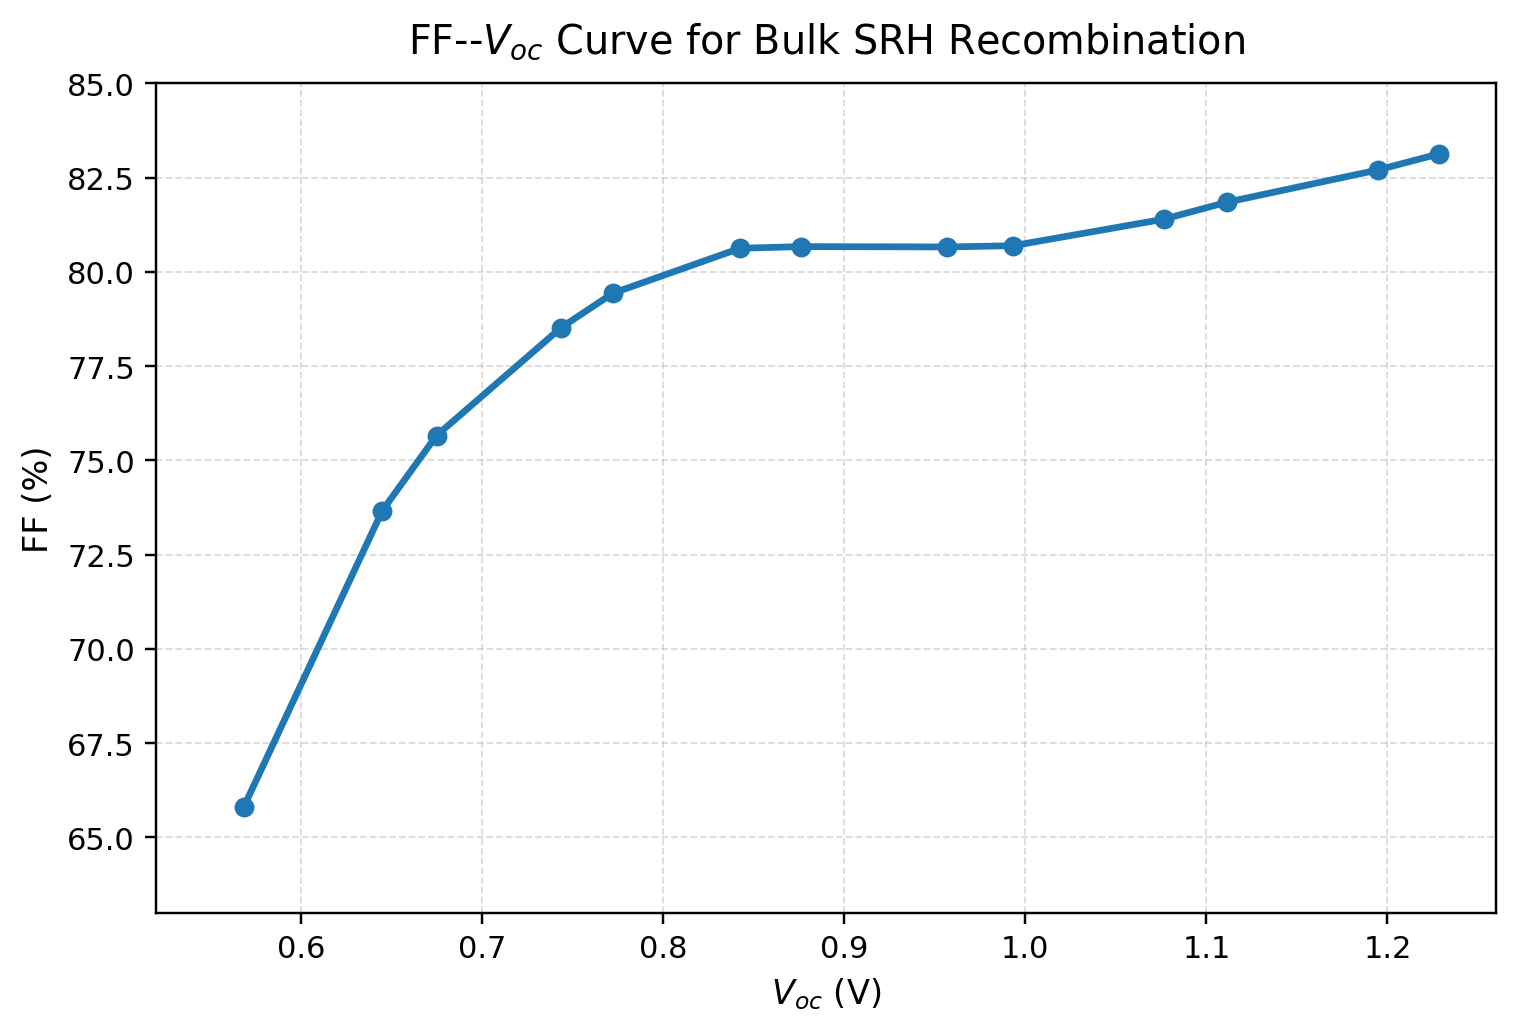
\includegraphics[width=0.82\textwidth]{q3_bulk_ff_voc.png}
    \caption{FF--$V_\mathrm{oc}$ curve for bulk SRH recombination}
    \label{fig:q3-bulk-ff-voc}
\end{figure}

\FloatBarrier

\subsubsection{Surface-SRH-Dominant Approximation Results}
Table \ref{tab:q3-surface} summarizes the surface-SRH-dominant approximation scan. The results show three regions:
\begin{enumerate}[label=\textbf{\arabic*.}]
    \item \textbf{Weak surface recombination:} from $10^2$ s to $10^0$ s, the points almost overlap at $V_\mathrm{oc}\approx1.3328$ V and FF $\approx87.9\%$.
    \item \textbf{Transition region:} near $10^{-4}$--$10^{-5}$ s, surface recombination starts to strongly influence the device, and FF drops sharply.
    \item \textbf{Strong surface recombination:} below $10^{-6}$ s, $V_\mathrm{oc}$ continues to decrease, while FF does not follow the same smooth trend as the bulk case.
\end{enumerate}

\begin{table}[H]
    \centering
    \caption{FF--$V_\mathrm{oc}$ data for the surface-SRH-dominant approximation scan}
    \label{tab:q3-surface}
    \small
    \begin{tabular}{@{}ccc@{}}
        \toprule
        Surface lifetime / s & $V_\mathrm{oc}$ / V & FF / \% \\
        \midrule
        $1\times10^{2}$ & 1.3328 & 87.8985 \\
        $1\times10^{1}$ & 1.3328 & 87.8985 \\
        $1\times10^{0}$ & 1.3328 & 87.8982 \\
        $1\times10^{-1}$ & 1.3328 & 87.8959 \\
        $1\times10^{-2}$ & 1.3328 & 87.8726 \\
        $1\times10^{-3}$ & 1.3328 & 87.6395 \\
        $1\times10^{-4}$ & 1.3300 & 85.5855 \\
        $1\times10^{-5}$ & 1.3104 & 76.0971 \\
        $1\times10^{-6}$ & 1.1004 & 79.8305 \\
        $1\times10^{-7}$ & 0.9562 & 82.6531 \\
        $1\times10^{-8}$ & 0.8568 & 83.4523 \\
        $1\times10^{-9}$ & 0.7756 & 82.4557 \\
        \bottomrule
    \end{tabular}
\end{table}

The separate surface-SRH-dominant FF--$V_\mathrm{oc}$ curve is shown in Figure \ref{fig:q3-surface-ff-voc}. Unlike the bulk case, the curve contains a high-$V_\mathrm{oc}$ plateau and a more complicated transition region, confirming that interface recombination changes the $J$--$V$ shape in a localized way.

\begin{figure}[H]
    \centering
    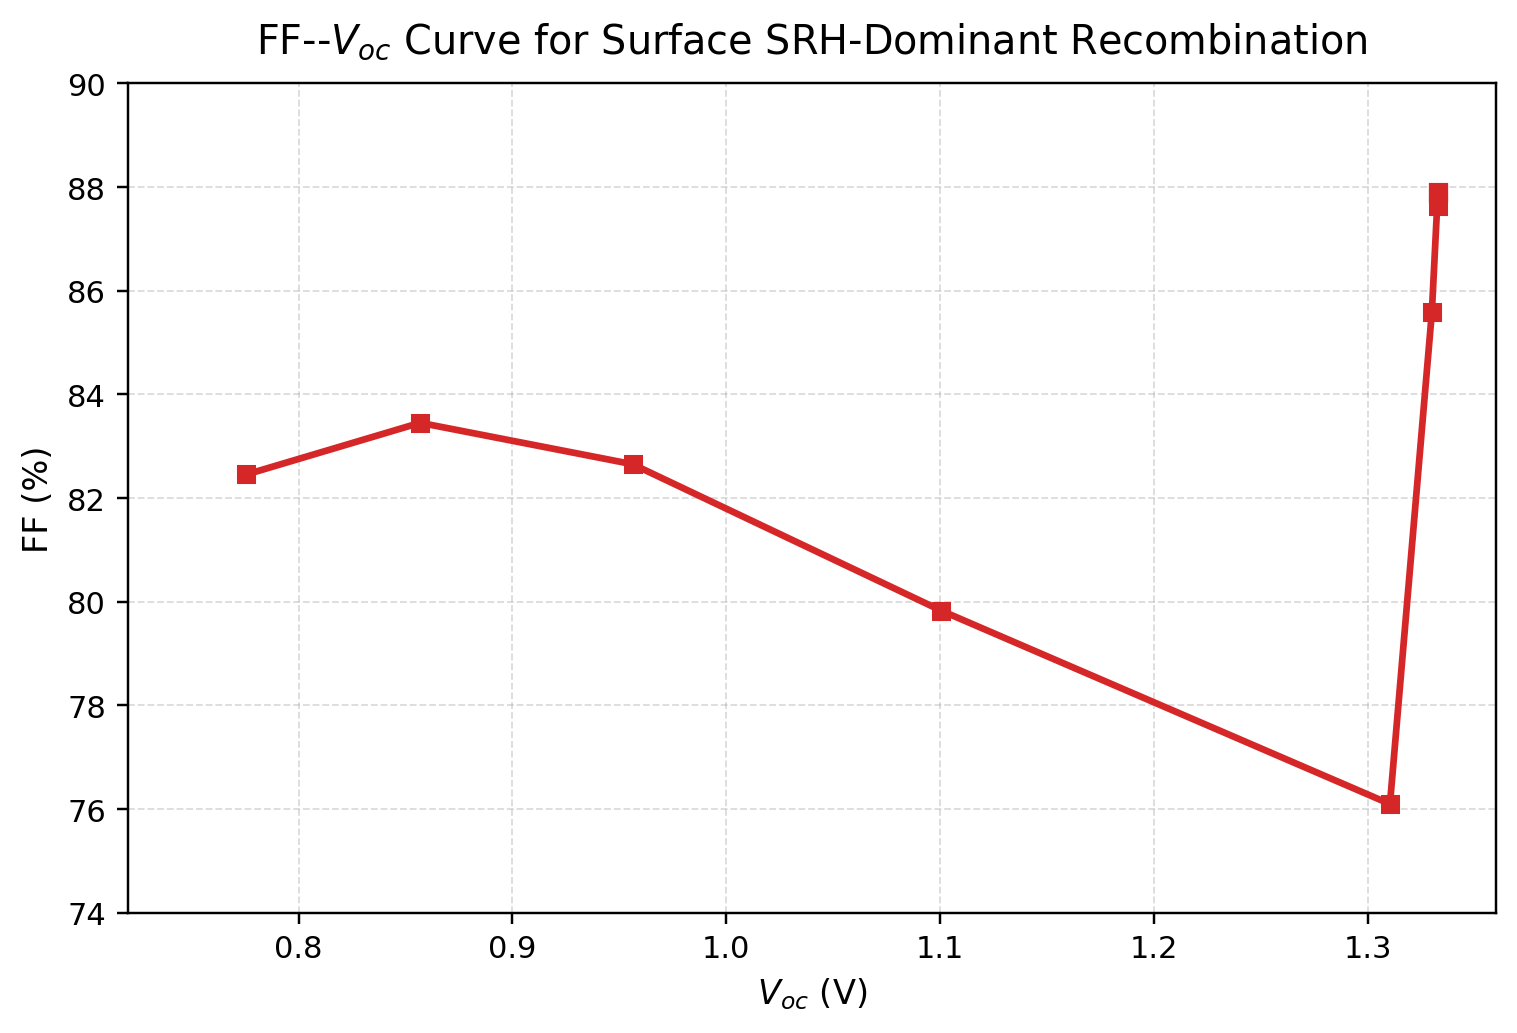
\includegraphics[width=0.82\textwidth]{q3_surface_ff_voc.png}
    \caption{FF--$V_\mathrm{oc}$ curve for the surface-SRH-dominant approximation}
    \label{fig:q3-surface-ff-voc}
\end{figure}

\FloatBarrier

\subsubsection{Comparison of the Two FF--$V_\mathrm{oc}$ Curves}
After examining the two mechanisms separately, Figure \ref{fig:q3-ff-voc} compares them in the same coordinate system. For bulk SRH recombination, FF decreases gradually and almost monotonically as $V_\mathrm{oc}$ decreases. For the surface-SRH-dominant approximation, the curve has a high-performance plateau and a stronger transition region. The key difference is that bulk recombination is distributed throughout the absorber, while surface recombination is localized at the interfaces.

\begin{figure}[H]
    \centering
    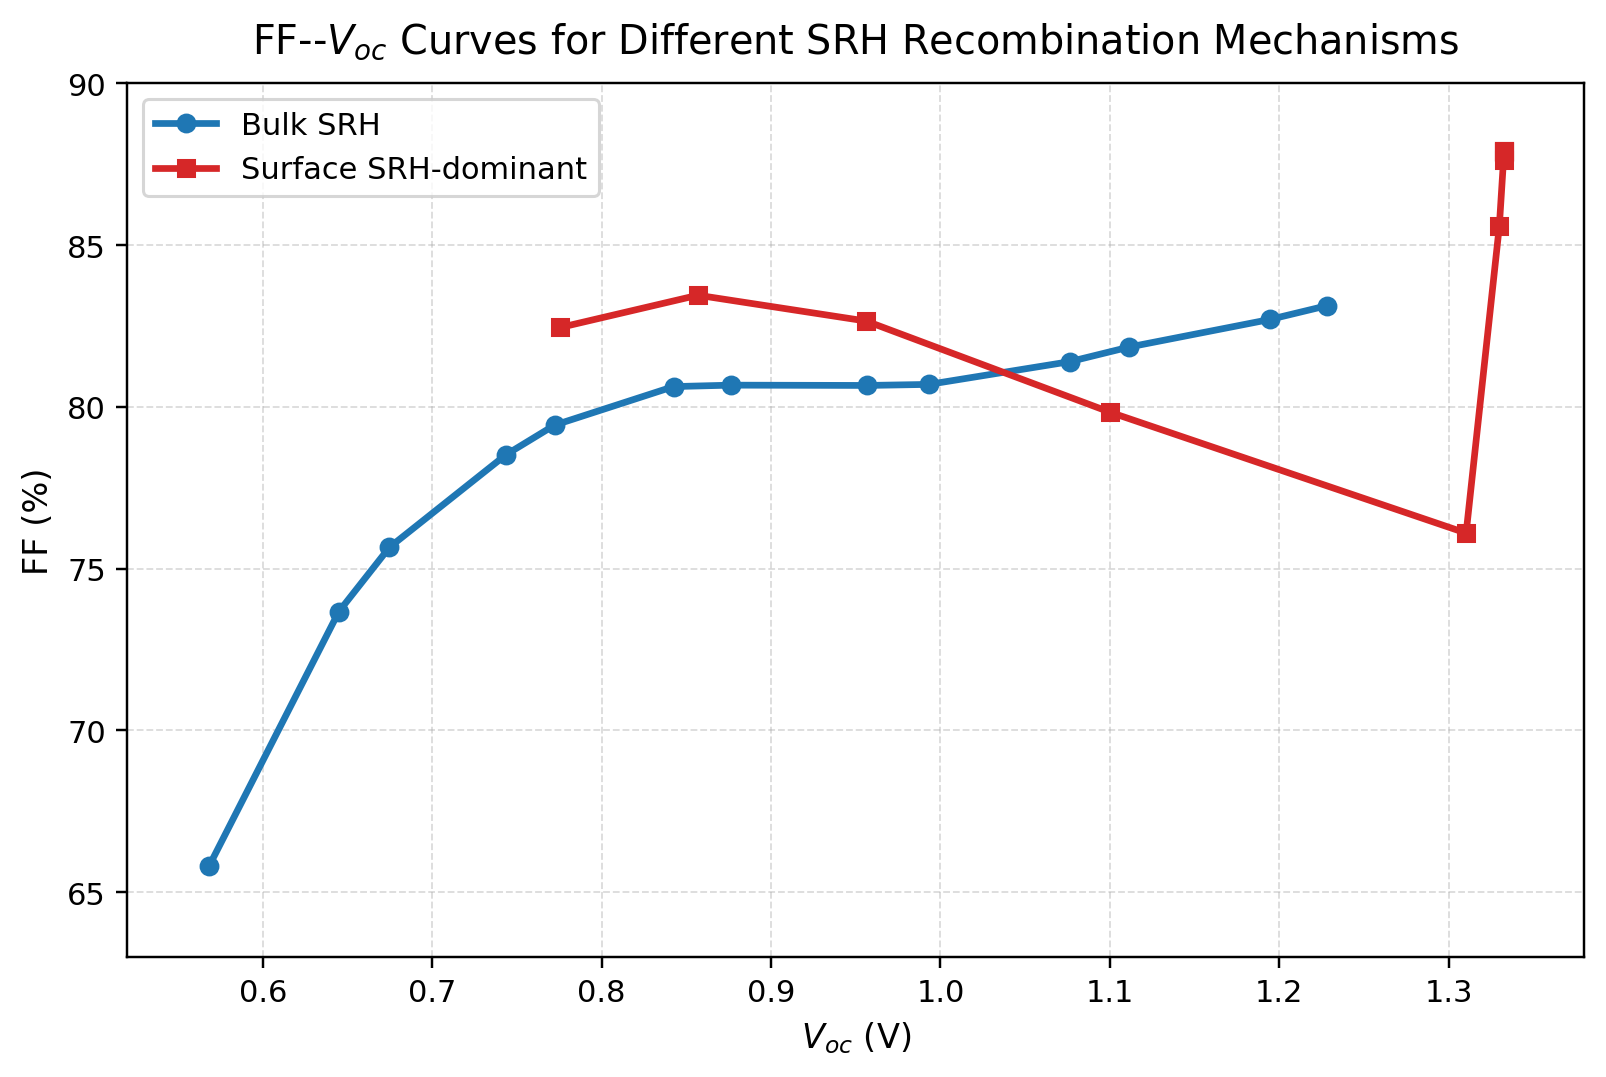
\includegraphics[width=0.82\textwidth]{q3_ff_voc_comparison.png}
    \caption{Comparison of FF--$V_\mathrm{oc}$ curves for bulk SRH and the surface-SRH-dominant approximation}
    \label{fig:q3-ff-voc}
\end{figure}

\FloatBarrier

The physical interpretation is:
\begin{enumerate}[label=\textbf{\arabic*.}]
    \item \textbf{Uniform bulk loss.}
    
    Shortening the bulk lifetime increases recombination throughout the active layer. This reduces both the quasi-Fermi-level splitting and the maximum-power output, so FF and $V_\mathrm{oc}$ decrease in a smooth coupled manner.

    \item \textbf{Localized interface loss.}
    
    Surface recombination directly affects carrier extraction at the interfaces. Therefore, it can distort the maximum-power region more strongly than uniform bulk recombination. This explains the pronounced FF loss around $V_\mathrm{oc}\approx1.31$ V.

    \item \textbf{Different FF--$V_\mathrm{oc}$ behavior.}
    
    The surface-SRH-dominant curve is not simply a shifted version of the bulk SRH curve. It reflects the fact that recombination location is also important, not only recombination strength.
\end{enumerate}

\clearpage
\begin{thebibliography}{99}

\bibitem{kojima2009}
A. Kojima, K. Teshima, Y. Shirai, and T. Miyasaka,
``Organometal halide perovskites as visible-light sensitizers for photovoltaic cells,''
\textit{Journal of the American Chemical Society}, vol. 131, no. 17, pp. 6050--6051, 2009.
doi: 10.1021/ja809598r.

\bibitem{stranks2013}
S. D. Stranks, G. E. Eperon, G. Grancini, C. Menelaou, M. J. P. Alcocer, T. Leijtens, L. M. Herz, A. Petrozza, and H. J. Snaith,
``Electron-hole diffusion lengths exceeding 1 micrometer in an organometal trihalide perovskite absorber,''
\textit{Science}, vol. 342, no. 6156, pp. 341--344, 2013.
doi: 10.1126/science.1243982.

\bibitem{dewolf2014}
S. De Wolf, J. Holovsky, S.-J. Moon, P. Loper, B. Niesen, M. Ledinsky, F.-J. Haug, J.-H. Yum, and C. Ballif,
``Organometallic halide perovskites: sharp optical absorption edge and its relation to photovoltaic performance,''
\textit{Journal of Physical Chemistry Letters}, vol. 5, no. 6, pp. 1035--1039, 2014.
doi: 10.1021/jz500279b.

\bibitem{green2016}
M. A. Green, K. Emery, Y. Hishikawa, W. Warta, and E. D. Dunlop,
``Solar cell efficiency tables (version 47),''
\textit{Progress in Photovoltaics: Research and Applications}, vol. 24, no. 1, pp. 3--11, 2016.
doi: 10.1002/pip.2728.

\bibitem{nelson2003}
J. Nelson,
\textit{The Physics of Solar Cells}.
London, UK: Imperial College Press, 2003.

\bibitem{pettersson1999}
L. A. A. Pettersson, L. S. Roman, and O. Inganas,
``Modeling photocurrent action spectra of photovoltaic devices based on organic thin films,''
\textit{Journal of Applied Physics}, vol. 86, no. 1, pp. 487--496, 1999.
doi: 10.1063/1.370757.

\bibitem{shockley1961}
W. Shockley and H. J. Queisser,
``Detailed balance limit of efficiency of p-n junction solar cells,''
\textit{Journal of Applied Physics}, vol. 32, no. 3, pp. 510--519, 1961.
doi: 10.1063/1.1736034.

\bibitem{shockley1952}
W. Shockley and W. T. Read,
``Statistics of the recombinations of holes and electrons,''
\textit{Physical Review}, vol. 87, no. 5, pp. 835--842, 1952.
doi: 10.1103/PhysRev.87.835.

\bibitem{hall1952}
R. N. Hall,
``Electron-hole recombination in germanium,''
\textit{Physical Review}, vol. 87, no. 2, p. 387, 1952.
doi: 10.1103/PhysRev.87.387.

\bibitem{tress2017}
W. Tress,
``Perovskite solar cells on the way to their radiative efficiency limit: insights into a success story of high open-circuit voltage and low recombination,''
\textit{Advanced Energy Materials}, vol. 7, no. 14, 1602358, 2017.
doi: 10.1002/aenm.201602358.

\bibitem{sze2007}
S. M. Sze and K. K. Ng,
\textit{Physics of Semiconductor Devices}, 3rd ed.
Hoboken, NJ, USA: Wiley-Interscience, 2007.

\end{thebibliography}

\clearpage
\appendix
\section{Supplementary Files}
The following supplementary files are included in the project folder. They record the extracted data and the plotting procedures used in this report.

\begin{table}[H]
    \centering
    \caption{Supplementary files for data processing and plotting}
    \small
    \begin{tabular}{@{}p{0.32\textwidth}p{0.60\textwidth}@{}}
        \toprule
        File & Description \\
        \midrule
        \texttt{q3.xlsx} & Extracted bulk and surface SRH scan data for Question 3 \\
        \texttt{plot\_q2\_thickness.py} & Python script for the four thickness-dependent curves in Question 2 \\
        \texttt{plot\_q3\_ff\_voc.py} & Python script for the FF--$V_\mathrm{oc}$ curves in Question 3 \\
        \texttt{figures/} & Original simulation screenshots and generated figures used in the report \\
        \bottomrule
    \end{tabular}
\end{table}

\begin{figure}[H]
    \centering
    \includegraphics[width=0.96\textwidth]{figure.png}
    \caption{Overview of the simulation screenshots, generated plots, and parameter files stored in the \texttt{figures/} folder}
    \label{fig:appendix-figures-overview}
\end{figure}

\FloatBarrier

\section{Python Code for Question 2}
\lstinputlisting[language=Python,caption={Python code for plotting the thickness dependence of photovoltaic parameters}]{plot_q2_thickness.py}

\section{Python Code for Question 3}
\lstinputlisting[language=Python,caption={Python code for plotting FF--$V_\mathrm{oc}$ curves under different SRH recombination mechanisms}]{plot_q3_ff_voc.py}

\end{document}
